
\section{Methodology}
\label{sec:methodology}
In this section, we will fully describe our approaches in conducting these latency related measurements.

\subsection{Latency in WAN}
\label{sec:latency-wan}
We derive our measurement methodology from King \cite{gummadi2002king} and Turbo-King \cite{leonard2008turbo}, and developed a Turbo-King variant illustrated in Fig.\,\ref{fig:king_model}. The King method leverages DNS name-servers to make measurements that approximate latency between arbitrary end hosts. It utilizes properties of DNS to coerce recursive DNS resolvers into making outbound queries on behalf of measuring party. Turbo-King builds upon King by allowing for detection of DNS forwarders. DNS forwarders aggregate DNS queries within a network that target external DNS servers and can serve responses. The original King method has no means of detecting these servers, and as a result they may skew measurement results.

Our methodology is composed of 4 elements, a measurement node, a central domain name server, and 2 target name servers. A measurement nodes is composed of a DNS client and server. A node accepts remote-procedure calls that specify 2 target DNS servers and returns both DNS latency measurements and multiple round trip time calculations to the first target server. The central domain name server simply refers incoming DNS requests to the originating measurement node. The 2 target name servers must have known locations and the first must be an open-recursive resolver. Below we outline the measurement process.

\begin{enumerate}
	\item DNS Client on measurement node will issue a request to the first target DNS server. The requested URL will be of the form "qid.myAddr.mydomain.com", where qid is the query id, myAddr is an encoding of the measurement nodes public name, and mydomain is the domain controlled our central name server.
	\item The target server will issue a request containing the requested URL to the central name server
	\item The central name server will decode the "myAddr" element of the requested URL to the url of the originating measurement node. It will return a response to the querying target server with a referral to the measurement node.
	\item The target name server will then issue a DNS query with the requested URL to the measurement node.
	\item The measurement node will receive a DNS query, lookup the query id and return a referral with the corresponding second target DNS server.
	\item The first target DNS server will issue a request to the second DNS server
	\item The second server will deliver a response (to be discussed more)
	\item The first target name server will then pass along this response to the DNS client of the measurement node.
\end{enumerate}

We record the time delta between step 5 and 8, and subtract the round-trip time between the measurement node and the first target to generate a latency measurement between the two target DNS servers. It is important to note that upon the first DNS request to the second target DNS server, that server itself may try a complete resolution if it is an open resolver. In this case, the second target server will issue a request to resolve our domain and will be referred to the originating measurement node. It will issue a request to this node that contains the original query id; in this event the measurement node will not issue a response and allow the second target server to time out. The second target will then return a NXDomain response to the first target name server, and upon subsequent requests for our domain (within some time period dictated by that servers caching policy) it will issue continue to issue error responses. Thus, we always discard the first latency measurement in every round to account for this additional lookup latency.

Finally, to determine the round trip latency between a measurement node and the first target server, we issue a DNS query for a random subdomain in the domain controlled by the target name server. We issue this request multiple times to allow and discard the first measurement. In this way we allow for the request to be cached on the target server and minimize the processing time to generate more accurate round-trip time measurements. We adopted This method is over ICMP ping because a fraction of DNS servers we queried did not respond to ICMP requests.

\begin{figure}
  \centering
  \includegraphics[width=\linewidth]{../figs/king_model.pdf}
  \caption{King/T-King method illustration}
  \label{fig:king_model}
\end{figure}



\subsection{Latency for DC conversations}
\label{sec:latency-dc-conv}
Bearing in mind that the primary goal for this part is to understand the partition of latency from end-users' perspective, we designed the experiment to perform data center related tasks. We expect the model in Fig.\,\ref{fig:DC_model} to be used, and the fractions in the WAN and the DC are also shown. 

\begin{figure}
  \centering
  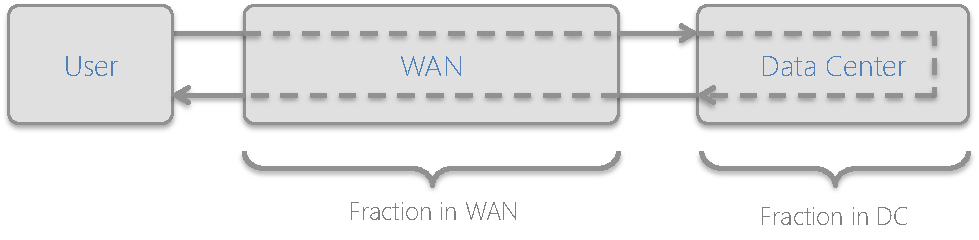
\includegraphics[width=\linewidth]{../figs/DC_model.pdf}
  \caption{Typical user-DC communication pattern}
  \label{fig:DC_model}
\end{figure}

As an representative user-facing service, we have chosen Google Search as the case study. One of the reason of choosing Google Search is that they provide an estimated time spent within their DC (Fig.\,\ref{fig:google_time}). From our analysis in Sec.\,\ref{sec:analysis}, this data is fairly accurate in reflecting the fraction in DC. 

\begin{figure}
  \centering
  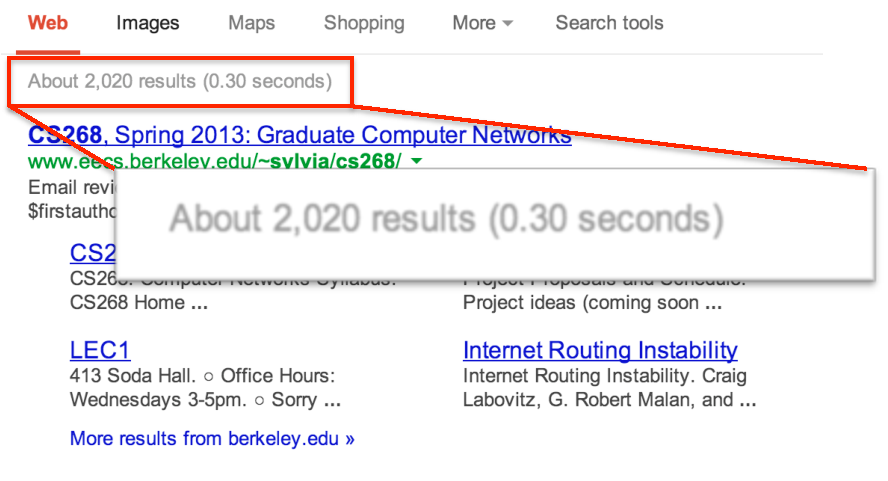
\includegraphics[width=0.85\linewidth]{../figs/GoogleTime.pdf}
  \caption{Google Search estimated time spent within Google in the return webpage}
  \label{fig:google_time}
\end{figure}

To measure the time for a single query, this can be easily done at the end-host side by timestamping the start and end of each query. But what to query remains a problem. Initially, we were suspecting that caching might happens at the Internet-facing router in DC. Querying the hottest words which are likely to be cached might reveal the WAN fraction. On the other side, to force the query to be processed by the DC (eliminating caching), we use random string for search. The hottest words can be found in Google Trends\footnote{http://www.google.com/trends/hottrends}, and we generate random strings comprised of lower cases, upper cases and numbers with length 32. Though the analysis in Sec.\,\ref{sec:analysis} shows a different results instead of what we have expected. This methodology is still useful to understand the problem we are initially planning to solve. 

In the meantime, {\it ping} is performed to measure the networking latency from the user to Google. Since we plan to conduct this experiment in geographically distributed fashion, and Google has many user-facing servers/IPs, we have to make sure we are measuring the right one. In this case, in additional to application layer HTTP conversation, we use {\it tcpdump} to capture all the packets and find out Google's IP address to ping.
 
In summary, to conduct the WAN vs. DC measurement, we issue query to Google and measure four different ``times'', shown in Table.\,\ref{tab:DC_method}.

\begin{table}
  \begin{tabular}{p{2.8cm} | p{5cm}}
    \hline
    type & description \\
    \hline
    Hot-trend-query time & the time spent to query a hot trend word to Google. \\
    Random-query time & the time spent to query a 32-character random string.  \\
    Ping time & the networking layer round-trip time to the responded Google IP address. \\
    Google time & Google's estimated time spent within their DC. \\
    \hline
  \end{tabular}
  \caption{Four different ``times'' measured}
  \label{tab:DC_method}
\end{table}

% \begin{itemize}
% \setlength{\leftmargin}{-1pt}
% \setlength{\itemsep}{1pt}
% \setlength{\parskip}{0pt}
% \setlength{\parsep}{0pt}
% \item Hot-trend-query time \\
%   the time spent to query a hot trend word to Google. 
% \item Random-query time -- the time spent to query a 32-character random string. 
% \item Ping time -- the networking layer round-trip time to the responded Google IP address.
% \item Google time -- Google's estimated time spent within their DC.
% \end{itemize}

\subsection{Latency within the Cellular Networks}
\label{sec:latency-with-celull}



%%% Local Variables: 
%%% mode: latex
%%% TeX-master: "main"
%%% End: 
